\documentclass{article}
\usepackage{tikz}
\usepackage[x11names, rgb]{xcolor}
\usepackage[a4paper, margin=0.5in]{geometry}
\usepackage{comment}

\usetikzlibrary{decorations.pathmorphing}
\tikzset{snake it/.style={decorate, decoration=snake}}

\begin{document}
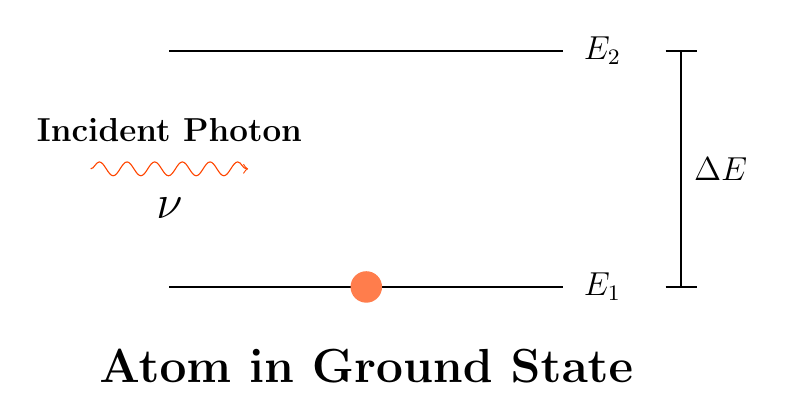
\begin{tikzpicture}

\definecolor{atom_red}{HTML}{FF4500}

\draw[thick] (0,3) -- (5,3);
\draw[thick] (0,0) -- (5,0);

\node at (5.5,3) {\textbf{\large $E_{2}$}};
\node at (5.5,0) {\textbf{\large $E_{1}$}};
\node at (7,1.5) {\textbf{\large $\Delta E$}};

\draw[thick] (6.5,3) -- (6.5,0);
\draw[thick] (6.3,3) -- (6.7,3);
\draw[thick] (6.3,0) -- (6.7,0);

% \begin{comment}

\draw[->, snake it, atom_red] (-1,1.5) -- (1,1.5);
\fill[atom_red!70] (2.5,0) circle (.2cm);

\node at (0, 2) {\textbf{\large Incident Photon}};
\node at (0, 1) {\textbf{\LARGE $\nu$}};
\node at (2.5, -1) {\textbf{\LARGE Atom in Ground State}};

% \end{comment}

\begin{comment}

\fill[atom_red!70] (2.5,3) circle (.2cm);
\fill[white] (2.5,0) circle (.2cm);
\draw[dashed] (2.5, 0) circle (.2cm);

\draw[thick, ->, >=latex] (2.5, 0.5) -- (2.5, 2.5);

\node at (2.5, 4) {\textbf{\LARGE Atom in Excited State}};

\end{comment}

\end{tikzpicture}
\end{document}
